\section{Выделение контура фигуры}
\label{sec:Edge}

Для выделения контура кисти руки можно использовать операторы преобразования изображения. К таким методам можно отнести:

\begin{itemize}
	\item Оператор Собеля \cite{Sobel}
	\item Оператор Прюитт \cite{Prewitt}
	\item Перекрестный оператор Робертса \cite{Roberts}
	\item Оператор Кэнни \cite{Canny}
\end{itemize}

Рассмотрим каждый подробнее:

\subsection{Оператор Собеля}

Основная идея оператора Собеля\cite{Sobel} заключается в вычислении градиента освещенности каждой точки изображения. Вычисление производится примерное с помощью свертки изображения двумя сепарабельными целочисленными фильтрами размера 3x3 в вертикальном и горизонтальном направлениях (рисунок \ref{fig:sobel}). Благодаря этому вычисление работа данного оператора имеет низкие трудозатраты. В результате получаются два новых изображения Gx и Gy, в каждой точке которого записано приближенное значение производных по x и по y соответственно. Пусть A - исходное изображение, тогда вычисляются они следующим образом:

\begin{eqnarray}\label{eq:sobel-matrixs}
G_x = \begin{bmatrix}
-1 & 0 & 1\\
-2 & 0 & 2\\
-1 & 0 & 1\\
\end{bmatrix} \\
G_y = \begin{bmatrix}
-1 & -2 & -1\\
0 & 0 & 0\\
1 & 2 & 1\\
\end{bmatrix}
\end{eqnarray}

\begin{figure*}[!h]
	\centering
	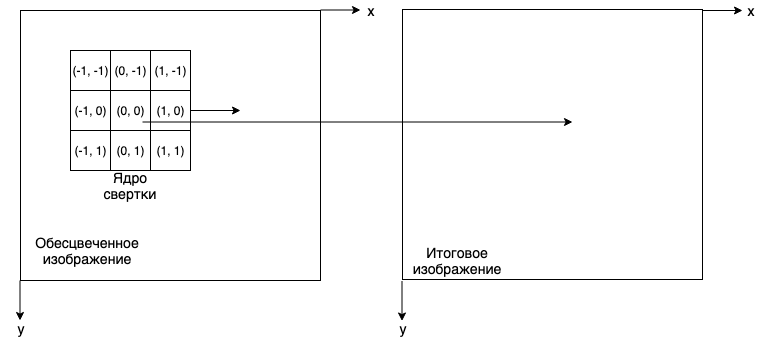
\includegraphics[width=\textwidth,keepaspectratio]{figures/ru/sobel.png}
	\caption{Свертка изображения для получения контура}
	\label{fig:sobel}
\end{figure*}

В итоге значение градиента вычисляется как $G=\sqrt{G_x^2+G_y^2}$, а его направление как $\theta=\arctan(\frac{G_x}{G_y})$.

Результат показывает скорость изменения яркости изображения в конкретной точке, т.е. вероятность ее нахождения на границе изображения.

\subsection{Оператор Прюитт}

Данный метод\cite{Prewitt}, как и оператор Собеля, использует свертку обесцвеченного изображения (рисунок \ref{fig:sobel}) ядром размера 3х3. Отличие заключается в способе задачи маски:

\begin{eqnarray}\label{eq:prewitt-matrixs}
G_x = \begin{bmatrix}
-1 & 0 & 1\\
-1 & 0 & 1\\
-1 & 0 & 1\\
\end{bmatrix} \\
G_y = \begin{bmatrix}
-1 & -1 & -1\\
0 & 0 & 0\\
1 & 1 & 1\\
\end{bmatrix}
\end{eqnarray}

Из-за меньшего значения средних элементов итоговое изображение имеет более явный эффект сглаживания.

\subsection{Перекрестный оператор Робертса}

Рассмотрим область 3х3, представленную ну рисунке \ref{fig:roberst}.

\begin{figure*}[!h]
	\centering
	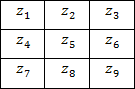
\includegraphics[width=0.2\textwidth,keepaspectratio]{figures/ru/roberts}
	\caption{Окрестность 3х3 внутри изображения}
	\label{fig:roberst}
\end{figure*}

Вычисление первых частных производных, которые обозначают перепад яркости, в точке $z_5$ можно провести следующим образом:

\begin{eqnarray}\label{eq:roberts-eq}
G_x = (z_9 - z_5) \\
G_y = (z_8 - z_6)
\end{eqnarray}

Для вычисления данных производных в каждой точке изображения в данном методе\cite{Roberts} применяется свертка изображения двумя ядрами размера 2х2:

\begin{eqnarray}\label{eq:roberts-matrixs}
\begin{bmatrix}
1 & 0\\
0 & -1
\end{bmatrix} 
\begin{bmatrix}
0 & 1\\
-1 & 0
\end{bmatrix}
\end{eqnarray}

В результате получается изображение пространственного градиента исходного изображения, где точки с наибольшим значением соответствуют границе.

Проблемой данного метода является отсутствие четко выраженного центрального элемента у ядра свертки. Но в следствии этого недостатка алгоритм так же имеет высокую скорость обработки изображения.

\subsection{Оператор Кэнни}

Данный фильтр\cite{Canny} был разработан с учетом удовлетворения следующих свойств:
\begin{itemize}
	\item хорошее обнаружение (Кэнни трактовал это свойство как повышение отношения сигнал/шум);
	\item хорошая локализация (правильное определение положения границы);
	\item единственный отклик на одну границу.
\end{itemize}

Алгоритм состоит из пяти последовательных шагов. Рассмотрим каждый из них подробнее с наглядной визуализацией обработки. Для этого применим данный оператор шаг за шагом к изображению \ref{fig:canny_orig}.

\begin{figure*}[!h]
	\centering
	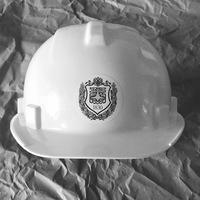
\includegraphics[width=0.2\textwidth,keepaspectratio]{figures/ru/bmstu_gray}
	\caption{Исходное изображение для обработки оператором Кэнни}
	\label{fig:canny_orig}
\end{figure*}

\begin{enumerate}
	\item Размытие изображения для удаления лишнего шума. Для этого можно применить фильтр Гаусса\cite{shapiro:2001}.
	Функция, используемая этим фильтром, для двумерного случая задается формулой  \ref{eq:gauss}.
	\begin{eqnarray}\label{eq:gauss}
	Gaus(x, y, \sigma) = \frac{1}{2 \pi \sigma^2}*e^{\frac{-(x^2+y^2)}{2\sigma^2}}
	\end{eqnarray}
	
	Результат применения фильтра Гаусса к изображению \ref{fig:canny_orig} представлен на рисунке \ref{fig:canny_smoothed}
	
	\begin{figure*}[!h]
		\centering
		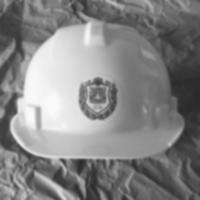
\includegraphics[width=0.2\textwidth,keepaspectratio]{figures/ru/bmstu_smoothed}
		\caption{Результат применения фильтра Гаусса}
		\label{fig:canny_smoothed}
	\end{figure*}
	\item Поиск градиентов, для определения границ с максимальным значением градиента.
	На данном этапе можно использовать оператор Собеля \cite{Sobel}, работа которого была описана выше.
	
	Результат поиска градиентов в размытом изображении представлен на рисунке \ref{fig:canny_gradient}.
	
	\begin{figure*}[!h]
		\centering
		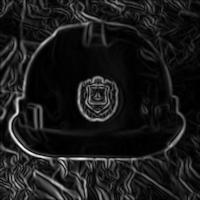
\includegraphics[width=0.2\textwidth,keepaspectratio]{figures/ru/bmstu_gradient}
		\caption{Результат поиска градиентов}
		\label{fig:canny_gradient}
	\end{figure*}

	\item Подавление не-максимумов, т.е. исключение из границ не локальных максимумов.
	
	На данном шаге происходит проверка, является ли конкретный пиксель локальным максимумом вдоль направления градиента. Таким образом исключаются ложные границы.
	
	\begin{figure*}[!h]
		\centering
		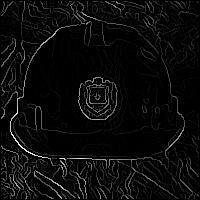
\includegraphics[width=0.2\textwidth,keepaspectratio]{figures/ru/bmstu_non_max}
		\caption{Изображение после подавления не-максимумов}
		\label{fig:canny_non_max}
	\end{figure*}

	\item Определение потенциальных границ с помощью двойной пороговой фильтрации.
	
	Фильтр использует два порога фильтрации:
	\begin{itemize}
		\item Все пиксели со значением больше верхней границы принимают максимальное значение (достоверная граница).
		\item Все пиксели со значением меньше нижней границы подавляются.
		\item Все пиксели со значением в диапазоне границ принимают фиксированное среднее значение. Их уточнение происходит на следующем этапе.
	\end{itemize}

	Пример фильтрации с порогами 0,01 и 0,07 представлен на рисунке \ref{fig:canny_threshold}.
	
	\begin{figure*}[!h]
		\centering
		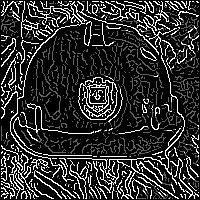
\includegraphics[width=0.2\textwidth,keepaspectratio]{figures/ru/bmstu_threshold}
		\caption{Результат двойной пороговой фильтрации}
		\label{fig:canny_threshold}
	\end{figure*}

	\item Трассировка области неоднозначности
	
	На данном этапе происходит разделение пикселей, получивших промежуточное значение на предыдущем шаге, на границы и фон (увеличение значения и подавление). Пиксель добавляется к границе, если он соприкасается с ней по одному из 8-ми направлений.
	
	Результат работы оператора Кэнни представлен на рисунке \ref{fig:canny_final}.
	
	\begin{figure*}[!h]
		\centering
		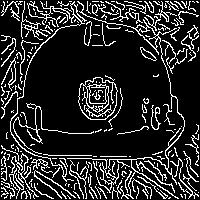
\includegraphics[width=0.2\textwidth,keepaspectratio]{figures/ru/bmstu_final}
		\caption{Результат работы оператора Кэнни}
		\label{fig:canny_final}
	\end{figure*}
\end{enumerate}


Стоит обратить внимание, что описанные выше методы принимают на вход изображение в серых тонах. То есть нулевым шагом данных методов можно указать преобразование изображения из цветного в черно-белое.
